% Created by tikzDevice version 0.12.3.1 on 2023-04-12 14:29:37
% !TEX encoding = UTF-8 Unicode
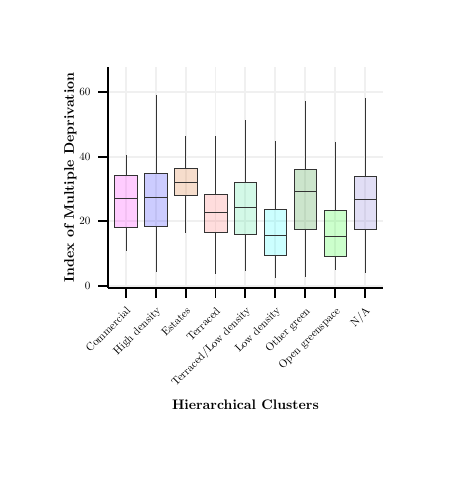
\begin{tikzpicture}[x=1pt,y=1pt]
\definecolor{fillColor}{RGB}{255,255,255}
\path[use as bounding box,fill=fillColor,fill opacity=0.00] (0,0) rectangle (142.64,152.15);
\begin{scope}
\path[clip] (  0.00,  0.00) rectangle (142.64,152.15);
\definecolor{fillColor}{RGB}{255,255,255}

\path[fill=fillColor] (  0.00,  0.00) rectangle (142.64,152.15);
\end{scope}
\begin{scope}
\path[clip] ( 28.95, 58.04) rectangle (128.41,137.92);
\definecolor{fillColor}{RGB}{255,255,255}

\path[fill=fillColor] ( 28.95, 58.04) rectangle (128.41,137.92);
\definecolor{drawColor}{gray}{0.94}

\path[draw=drawColor,line width= 0.7pt,line join=round] ( 28.95, 58.96) --
	(128.41, 58.96);

\path[draw=drawColor,line width= 0.7pt,line join=round] ( 28.95, 82.25) --
	(128.41, 82.25);

\path[draw=drawColor,line width= 0.7pt,line join=round] ( 28.95,105.55) --
	(128.41,105.55);

\path[draw=drawColor,line width= 0.7pt,line join=round] ( 28.95,128.84) --
	(128.41,128.84);

\path[draw=drawColor,line width= 0.7pt,line join=round] ( 35.43, 58.04) --
	( 35.43,137.92);

\path[draw=drawColor,line width= 0.7pt,line join=round] ( 46.25, 58.04) --
	( 46.25,137.92);

\path[draw=drawColor,line width= 0.7pt,line join=round] ( 57.06, 58.04) --
	( 57.06,137.92);

\path[draw=drawColor,line width= 0.7pt,line join=round] ( 67.87, 58.04) --
	( 67.87,137.92);

\path[draw=drawColor,line width= 0.7pt,line join=round] ( 78.68, 58.04) --
	( 78.68,137.92);

\path[draw=drawColor,line width= 0.7pt,line join=round] ( 89.49, 58.04) --
	( 89.49,137.92);

\path[draw=drawColor,line width= 0.7pt,line join=round] (100.30, 58.04) --
	(100.30,137.92);

\path[draw=drawColor,line width= 0.7pt,line join=round] (111.11, 58.04) --
	(111.11,137.92);

\path[draw=drawColor,line width= 0.7pt,line join=round] (121.93, 58.04) --
	(121.93,137.92);
\definecolor{drawColor}{gray}{0.20}

\path[draw=drawColor,line width= 0.1pt,line join=round] ( 46.25, 99.60) -- ( 46.25,127.69);

\path[draw=drawColor,line width= 0.1pt,line join=round] ( 46.25, 80.42) -- ( 46.25, 63.99);
\definecolor{fillColor}{RGB}{0,0,255}

\path[draw=drawColor,line width= 0.1pt,fill=fillColor,fill opacity=0.20] ( 42.19, 99.60) --
	( 42.19, 80.42) --
	( 50.30, 80.42) --
	( 50.30, 99.60) --
	( 42.19, 99.60) --
	cycle;

\path[draw=drawColor,line width= 0.1pt] ( 42.19, 90.93) -- ( 50.30, 90.93);

\path[draw=drawColor,line width= 0.1pt,line join=round] ( 35.43, 98.85) -- ( 35.43,106.18);

\path[draw=drawColor,line width= 0.1pt,line join=round] ( 35.43, 80.15) -- ( 35.43, 71.61);
\definecolor{fillColor}{RGB}{255,0,255}

\path[draw=drawColor,line width= 0.1pt,fill=fillColor,fill opacity=0.20] ( 31.38, 98.85) --
	( 31.38, 80.15) --
	( 39.49, 80.15) --
	( 39.49, 98.85) --
	( 31.38, 98.85) --
	cycle;

\path[draw=drawColor,line width= 0.1pt] ( 31.38, 90.59) -- ( 39.49, 90.59);

\path[draw=drawColor,line width= 0.1pt,line join=round] ( 89.49, 86.45) -- ( 89.49,111.05);

\path[draw=drawColor,line width= 0.1pt,line join=round] ( 89.49, 70.05) -- ( 89.49, 61.67);
\definecolor{fillColor}{RGB}{0,255,255}

\path[draw=drawColor,line width= 0.1pt,fill=fillColor,fill opacity=0.20] ( 85.44, 86.45) --
	( 85.44, 70.05) --
	( 93.55, 70.05) --
	( 93.55, 86.45) --
	( 85.44, 86.45) --
	cycle;

\path[draw=drawColor,line width= 0.1pt] ( 85.44, 77.22) -- ( 93.55, 77.22);

\path[draw=drawColor,line width= 0.1pt,line join=round] (100.30,101.11) -- (100.30,125.63);

\path[draw=drawColor,line width= 0.1pt,line join=round] (100.30, 79.49) -- (100.30, 62.16);
\definecolor{fillColor}{RGB}{0,128,0}

\path[draw=drawColor,line width= 0.1pt,fill=fillColor,fill opacity=0.20] ( 96.25,101.11) --
	( 96.25, 79.49) --
	(104.36, 79.49) --
	(104.36,101.11) --
	( 96.25,101.11) --
	cycle;

\path[draw=drawColor,line width= 0.1pt] ( 96.25, 93.01) -- (104.36, 93.01);

\path[draw=drawColor,line width= 0.1pt,line join=round] ( 67.87, 92.05) -- ( 67.87,112.95);

\path[draw=drawColor,line width= 0.1pt,line join=round] ( 67.87, 78.10) -- ( 67.87, 63.12);
\definecolor{fillColor}{RGB}{255,85,85}

\path[draw=drawColor,line width= 0.1pt,fill=fillColor,fill opacity=0.20] ( 63.81, 92.05) --
	( 63.81, 78.10) --
	( 71.92, 78.10) --
	( 71.92, 92.05) --
	( 63.81, 92.05) --
	cycle;

\path[draw=drawColor,line width= 0.1pt] ( 63.81, 85.55) -- ( 71.92, 85.55);

\path[draw=drawColor,line width= 0.1pt,line join=round] ( 78.68, 96.26) -- ( 78.68,118.85);

\path[draw=drawColor,line width= 0.1pt,line join=round] ( 78.68, 77.42) -- ( 78.68, 64.18);
\definecolor{fillColor}{RGB}{37,229,137}

\path[draw=drawColor,line width= 0.1pt,fill=fillColor,fill opacity=0.20] ( 74.63, 96.26) --
	( 74.63, 77.42) --
	( 82.73, 77.42) --
	( 82.73, 96.26) --
	( 74.63, 96.26) --
	cycle;

\path[draw=drawColor,line width= 0.1pt] ( 74.63, 87.36) -- ( 82.73, 87.36);

\path[draw=drawColor,line width= 0.1pt,line join=round] (111.11, 86.20) -- (111.11,110.98);

\path[draw=drawColor,line width= 0.1pt,line join=round] (111.11, 69.68) -- (111.11, 64.43);
\definecolor{fillColor}{RGB}{0,255,0}

\path[draw=drawColor,line width= 0.1pt,fill=fillColor,fill opacity=0.20] (107.06, 86.20) --
	(107.06, 69.68) --
	(115.17, 69.68) --
	(115.17, 86.20) --
	(107.06, 86.20) --
	cycle;

\path[draw=drawColor,line width= 0.1pt] (107.06, 76.86) -- (115.17, 76.86);

\path[draw=drawColor,line width= 0.1pt,line join=round] ( 57.06,101.28) -- ( 57.06,113.07);

\path[draw=drawColor,line width= 0.1pt,line join=round] ( 57.06, 91.52) -- ( 57.06, 77.97);
\definecolor{fillColor}{RGB}{212,85,0}

\path[draw=drawColor,line width= 0.1pt,fill=fillColor,fill opacity=0.20] ( 53.00,101.28) --
	( 53.00, 91.52) --
	( 61.11, 91.52) --
	( 61.11,101.28) --
	( 53.00,101.28) --
	cycle;

\path[draw=drawColor,line width= 0.1pt] ( 53.00, 96.40) -- ( 61.11, 96.40);

\path[draw=drawColor,line width= 0.1pt,line join=round] (121.93, 98.68) -- (121.93,126.71);

\path[draw=drawColor,line width= 0.1pt,line join=round] (121.93, 79.34) -- (121.93, 63.36);
\definecolor{fillColor}{RGB}{106,90,205}

\path[draw=drawColor,line width= 0.1pt,fill=fillColor,fill opacity=0.20] (117.87, 98.68) --
	(117.87, 79.34) --
	(125.98, 79.34) --
	(125.98, 98.68) --
	(117.87, 98.68) --
	cycle;

\path[draw=drawColor,line width= 0.1pt] (117.87, 90.25) -- (125.98, 90.25);

\path[] ( 28.95, 58.04) rectangle (128.41,137.92);
\end{scope}
\begin{scope}
\path[clip] (  0.00,  0.00) rectangle (142.64,152.15);
\definecolor{drawColor}{RGB}{0,0,0}

\path[draw=drawColor,line width= 0.7pt,line join=round] ( 28.95, 58.04) --
	( 28.95,137.92);
\end{scope}
\begin{scope}
\path[clip] (  0.00,  0.00) rectangle (142.64,152.15);
\definecolor{drawColor}{RGB}{0,0,0}

\node[text=drawColor,anchor=base east,inner sep=0pt, outer sep=0pt, scale=  0.40] at ( 22.65, 57.58) {0};

\node[text=drawColor,anchor=base east,inner sep=0pt, outer sep=0pt, scale=  0.40] at ( 22.65, 80.88) {20};

\node[text=drawColor,anchor=base east,inner sep=0pt, outer sep=0pt, scale=  0.40] at ( 22.65,104.17) {40};

\node[text=drawColor,anchor=base east,inner sep=0pt, outer sep=0pt, scale=  0.40] at ( 22.65,127.47) {60};
\end{scope}
\begin{scope}
\path[clip] (  0.00,  0.00) rectangle (142.64,152.15);
\definecolor{drawColor}{RGB}{0,0,0}

\path[draw=drawColor,line width= 0.7pt,line join=round] ( 25.45, 58.96) --
	( 28.95, 58.96);

\path[draw=drawColor,line width= 0.7pt,line join=round] ( 25.45, 82.25) --
	( 28.95, 82.25);

\path[draw=drawColor,line width= 0.7pt,line join=round] ( 25.45,105.55) --
	( 28.95,105.55);

\path[draw=drawColor,line width= 0.7pt,line join=round] ( 25.45,128.84) --
	( 28.95,128.84);
\end{scope}
\begin{scope}
\path[clip] (  0.00,  0.00) rectangle (142.64,152.15);
\definecolor{drawColor}{RGB}{0,0,0}

\path[draw=drawColor,line width= 0.7pt,line join=round] ( 28.95, 58.04) --
	(128.41, 58.04);
\end{scope}
\begin{scope}
\path[clip] (  0.00,  0.00) rectangle (142.64,152.15);
\definecolor{drawColor}{RGB}{0,0,0}

\path[draw=drawColor,line width= 0.7pt,line join=round] ( 35.43, 54.54) --
	( 35.43, 58.04);

\path[draw=drawColor,line width= 0.7pt,line join=round] ( 46.25, 54.54) --
	( 46.25, 58.04);

\path[draw=drawColor,line width= 0.7pt,line join=round] ( 57.06, 54.54) --
	( 57.06, 58.04);

\path[draw=drawColor,line width= 0.7pt,line join=round] ( 67.87, 54.54) --
	( 67.87, 58.04);

\path[draw=drawColor,line width= 0.7pt,line join=round] ( 78.68, 54.54) --
	( 78.68, 58.04);

\path[draw=drawColor,line width= 0.7pt,line join=round] ( 89.49, 54.54) --
	( 89.49, 58.04);

\path[draw=drawColor,line width= 0.7pt,line join=round] (100.30, 54.54) --
	(100.30, 58.04);

\path[draw=drawColor,line width= 0.7pt,line join=round] (111.11, 54.54) --
	(111.11, 58.04);

\path[draw=drawColor,line width= 0.7pt,line join=round] (121.93, 54.54) --
	(121.93, 58.04);
\end{scope}
\begin{scope}
\path[clip] (  0.00,  0.00) rectangle (142.64,152.15);
\definecolor{drawColor}{RGB}{0,0,0}

\node[text=drawColor,rotate= 45.00,anchor=base east,inner sep=0pt, outer sep=0pt, scale=  0.40] at ( 37.36, 49.51) {Commercial};

\node[text=drawColor,rotate= 45.00,anchor=base east,inner sep=0pt, outer sep=0pt, scale=  0.40] at ( 48.17, 49.51) {High density};

\node[text=drawColor,rotate= 45.00,anchor=base east,inner sep=0pt, outer sep=0pt, scale=  0.40] at ( 58.99, 49.51) {Estates};

\node[text=drawColor,rotate= 45.00,anchor=base east,inner sep=0pt, outer sep=0pt, scale=  0.40] at ( 69.80, 49.51) {Terraced};

\node[text=drawColor,rotate= 45.00,anchor=base east,inner sep=0pt, outer sep=0pt, scale=  0.40] at ( 80.61, 49.51) {Terraced/Low density};

\node[text=drawColor,rotate= 45.00,anchor=base east,inner sep=0pt, outer sep=0pt, scale=  0.40] at ( 91.42, 49.51) {Low density};

\node[text=drawColor,rotate= 45.00,anchor=base east,inner sep=0pt, outer sep=0pt, scale=  0.40] at (102.23, 49.51) {Other green};

\node[text=drawColor,rotate= 45.00,anchor=base east,inner sep=0pt, outer sep=0pt, scale=  0.40] at (113.04, 49.51) {Open greenspace};

\node[text=drawColor,rotate= 45.00,anchor=base east,inner sep=0pt, outer sep=0pt, scale=  0.40] at (123.85, 49.51) {N/A};
\end{scope}
\begin{scope}
\path[clip] (  0.00,  0.00) rectangle (142.64,152.15);
\definecolor{drawColor}{RGB}{0,0,0}

\node[text=drawColor,anchor=base,inner sep=0pt, outer sep=0pt, scale=  0.50] at ( 78.68, 14.03) {\bfseries Hierarchical Clusters};
\end{scope}
\begin{scope}
\path[clip] (  0.00,  0.00) rectangle (142.64,152.15);
\definecolor{drawColor}{RGB}{0,0,0}

\node[text=drawColor,rotate= 90.00,anchor=base,inner sep=0pt, outer sep=0pt, scale=  0.50] at ( 16.70, 97.98) {\bfseries Index of Multiple Deprivation};
\end{scope}
\end{tikzpicture}
